\documentclass[tikz]{standalone}
\usepackage{pgfplots}
\pgfplotsset{compat=1.15}
\usepackage{mathrsfs}
\usetikzlibrary{arrows,calc}
\usepackage{tkz-euclide}

\pagestyle{empty}

\definecolor{AngleClr}{rgb}{0,0.39215686274509803,0}
\definecolor{ShapeClr}{rgb}{0.6,0.2,0}
\definecolor{ParacircleClr}{RGB}{217,185,7}
\definecolor{BlueSqr}{RGB}{5,81,163}

\begin{document}

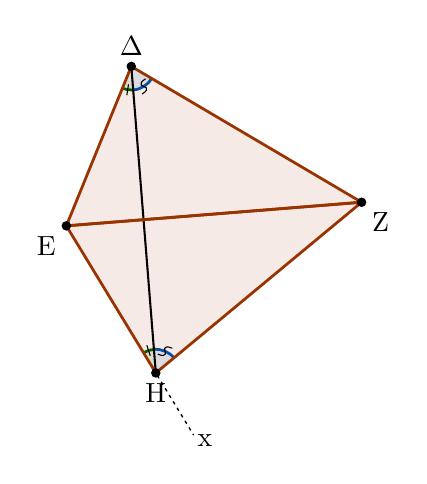
\begin{tikzpicture}[scale=.75]
\tkzSetUpLine[line width=1pt,color=black]
\tkzSetUpPoint[fill=black]

\tkzDefPoints{0/0/E,1.1/2.7/D,5/0.4/Z}

\tkzDefPointBy[reflection = over E--Z](D)\tkzGetPoint{H}
\tkzDefPointOnLine[pos=1.35](E,H)\tkzGetPoint{x}

\tkzFillPolygon[fill=ShapeClr,fill opacity=0.1](D,E,Z)
\tkzFillPolygon[fill=ShapeClr,fill opacity=0.1](E,Z,H)

\tkzFillAngle[fill=AngleClr,size=.4,fill opacity=0.1](E,D,H)
\tkzMarkAngle[mark=|,mksize=2,line width=1pt,color=AngleClr,size=.4](E,D,H)

\tkzFillAngle[fill=AngleClr,size=.4,fill opacity=0.1](D,H,E)
\tkzMarkAngle[mark=|,mksize=2,line width=1pt,color=AngleClr,size=.4](D,H,E)

\tkzFillAngle[fill=BlueSqr,size=.4,fill opacity=0.1](H,D,Z)
\tkzMarkAngle[mark=s,mksize=2,line width=1pt,color=BlueSqr,size=.4](H,D,Z)

\tkzFillAngle[fill=BlueSqr,size=.4,fill opacity=0.1](Z,H,D)
\tkzMarkAngle[mark=s,mksize=2,line width=1pt,color=BlueSqr,size=.4](Z,H,D)

\tkzDrawSegments[line width=0.75pt,color=black](D,H)

\tkzDrawLines[line width=0.5pt,dashed,dash pattern=on 1pt off 1.75pt](H,x)

\tkzDrawPolygon[color=ShapeClr](D,E,Z)
\tkzDrawPolygon[color=ShapeClr](E,Z,H)

\tkzDrawPoints[size=3](D,E,Z,H)

\tkzLabelPoint[above](D){$\rm \Delta$}
\tkzLabelPoint[below left](E){$\rm E$}
\tkzLabelPoint[below right](Z){$\rm Z$}
\tkzLabelPoint[below](H){$\rm H$}
\tkzLabelPoint[below right](x){$\rm x$}

\end{tikzpicture}
\end{document}
